% Options for packages loaded elsewhere
\PassOptionsToPackage{unicode}{hyperref}
\PassOptionsToPackage{hyphens}{url}
%
\documentclass[
]{article}
\usepackage{amsmath,amssymb}
\usepackage{iftex}
\ifPDFTeX
  \usepackage[T1]{fontenc}
  \usepackage[utf8]{inputenc}
  \usepackage{textcomp} % provide euro and other symbols
\else % if luatex or xetex
  \usepackage{unicode-math} % this also loads fontspec
  \defaultfontfeatures{Scale=MatchLowercase}
  \defaultfontfeatures[\rmfamily]{Ligatures=TeX,Scale=1}
\fi
\usepackage{lmodern}
\ifPDFTeX\else
  % xetex/luatex font selection
\fi
% Use upquote if available, for straight quotes in verbatim environments
\IfFileExists{upquote.sty}{\usepackage{upquote}}{}
\IfFileExists{microtype.sty}{% use microtype if available
  \usepackage[]{microtype}
  \UseMicrotypeSet[protrusion]{basicmath} % disable protrusion for tt fonts
}{}
\makeatletter
\@ifundefined{KOMAClassName}{% if non-KOMA class
  \IfFileExists{parskip.sty}{%
    \usepackage{parskip}
  }{% else
    \setlength{\parindent}{0pt}
    \setlength{\parskip}{6pt plus 2pt minus 1pt}}
}{% if KOMA class
  \KOMAoptions{parskip=half}}
\makeatother
\usepackage{xcolor}
\usepackage[margin=1in]{geometry}
\usepackage{color}
\usepackage{fancyvrb}
\newcommand{\VerbBar}{|}
\newcommand{\VERB}{\Verb[commandchars=\\\{\}]}
\DefineVerbatimEnvironment{Highlighting}{Verbatim}{commandchars=\\\{\}}
% Add ',fontsize=\small' for more characters per line
\usepackage{framed}
\definecolor{shadecolor}{RGB}{248,248,248}
\newenvironment{Shaded}{\begin{snugshade}}{\end{snugshade}}
\newcommand{\AlertTok}[1]{\textcolor[rgb]{0.94,0.16,0.16}{#1}}
\newcommand{\AnnotationTok}[1]{\textcolor[rgb]{0.56,0.35,0.01}{\textbf{\textit{#1}}}}
\newcommand{\AttributeTok}[1]{\textcolor[rgb]{0.13,0.29,0.53}{#1}}
\newcommand{\BaseNTok}[1]{\textcolor[rgb]{0.00,0.00,0.81}{#1}}
\newcommand{\BuiltInTok}[1]{#1}
\newcommand{\CharTok}[1]{\textcolor[rgb]{0.31,0.60,0.02}{#1}}
\newcommand{\CommentTok}[1]{\textcolor[rgb]{0.56,0.35,0.01}{\textit{#1}}}
\newcommand{\CommentVarTok}[1]{\textcolor[rgb]{0.56,0.35,0.01}{\textbf{\textit{#1}}}}
\newcommand{\ConstantTok}[1]{\textcolor[rgb]{0.56,0.35,0.01}{#1}}
\newcommand{\ControlFlowTok}[1]{\textcolor[rgb]{0.13,0.29,0.53}{\textbf{#1}}}
\newcommand{\DataTypeTok}[1]{\textcolor[rgb]{0.13,0.29,0.53}{#1}}
\newcommand{\DecValTok}[1]{\textcolor[rgb]{0.00,0.00,0.81}{#1}}
\newcommand{\DocumentationTok}[1]{\textcolor[rgb]{0.56,0.35,0.01}{\textbf{\textit{#1}}}}
\newcommand{\ErrorTok}[1]{\textcolor[rgb]{0.64,0.00,0.00}{\textbf{#1}}}
\newcommand{\ExtensionTok}[1]{#1}
\newcommand{\FloatTok}[1]{\textcolor[rgb]{0.00,0.00,0.81}{#1}}
\newcommand{\FunctionTok}[1]{\textcolor[rgb]{0.13,0.29,0.53}{\textbf{#1}}}
\newcommand{\ImportTok}[1]{#1}
\newcommand{\InformationTok}[1]{\textcolor[rgb]{0.56,0.35,0.01}{\textbf{\textit{#1}}}}
\newcommand{\KeywordTok}[1]{\textcolor[rgb]{0.13,0.29,0.53}{\textbf{#1}}}
\newcommand{\NormalTok}[1]{#1}
\newcommand{\OperatorTok}[1]{\textcolor[rgb]{0.81,0.36,0.00}{\textbf{#1}}}
\newcommand{\OtherTok}[1]{\textcolor[rgb]{0.56,0.35,0.01}{#1}}
\newcommand{\PreprocessorTok}[1]{\textcolor[rgb]{0.56,0.35,0.01}{\textit{#1}}}
\newcommand{\RegionMarkerTok}[1]{#1}
\newcommand{\SpecialCharTok}[1]{\textcolor[rgb]{0.81,0.36,0.00}{\textbf{#1}}}
\newcommand{\SpecialStringTok}[1]{\textcolor[rgb]{0.31,0.60,0.02}{#1}}
\newcommand{\StringTok}[1]{\textcolor[rgb]{0.31,0.60,0.02}{#1}}
\newcommand{\VariableTok}[1]{\textcolor[rgb]{0.00,0.00,0.00}{#1}}
\newcommand{\VerbatimStringTok}[1]{\textcolor[rgb]{0.31,0.60,0.02}{#1}}
\newcommand{\WarningTok}[1]{\textcolor[rgb]{0.56,0.35,0.01}{\textbf{\textit{#1}}}}
\usepackage{graphicx}
\makeatletter
\def\maxwidth{\ifdim\Gin@nat@width>\linewidth\linewidth\else\Gin@nat@width\fi}
\def\maxheight{\ifdim\Gin@nat@height>\textheight\textheight\else\Gin@nat@height\fi}
\makeatother
% Scale images if necessary, so that they will not overflow the page
% margins by default, and it is still possible to overwrite the defaults
% using explicit options in \includegraphics[width, height, ...]{}
\setkeys{Gin}{width=\maxwidth,height=\maxheight,keepaspectratio}
% Set default figure placement to htbp
\makeatletter
\def\fps@figure{htbp}
\makeatother
\setlength{\emergencystretch}{3em} % prevent overfull lines
\providecommand{\tightlist}{%
  \setlength{\itemsep}{0pt}\setlength{\parskip}{0pt}}
\setcounter{secnumdepth}{-\maxdimen} % remove section numbering
\ifLuaTeX
  \usepackage{selnolig}  % disable illegal ligatures
\fi
\usepackage{bookmark}
\IfFileExists{xurl.sty}{\usepackage{xurl}}{} % add URL line breaks if available
\urlstyle{same}
\hypersetup{
  pdftitle={Looping},
  pdfauthor={Naomi Tague},
  hidelinks,
  pdfcreator={LaTeX via pandoc}}

\title{Looping}
\author{Naomi Tague}
\date{January, 2025}

\begin{document}
\maketitle

\section{A more complex example of looping in
R}\label{a-more-complex-example-of-looping-in-r}

\subsubsection{Note, I edited this RMD with the required changes for HW
\#4}\label{note-i-edited-this-rmd-with-the-required-changes-for-hw-4}

Lets \textbf{scale} up from a single car to a group of cars on a highway
and use our \textbf{autopower} function to estimate a distribution of
power

What might vary?

\section{Our highway}\label{our-highway}

4 car types

Imagine with have 3 different car types - and we know how often each
occurs:

\begin{itemize}
\item
  car A mass 20000 kg, area 22 m\textsuperscript{2}
\item
  car B mass 65000 kg, area 30 m\textsuperscript{2}
\item
  car C mass 38000 kg area 22 m\textsuperscript{2}
\item
  car D mass 5000 kg area 10 m\textsuperscript{2}
\end{itemize}

Mean highway speed is 80 km/hr

\begin{Shaded}
\begin{Highlighting}[]
\FunctionTok{source}\NormalTok{(}\StringTok{"../ESM262\_HW4/autopower.R"}\NormalTok{)}
\CommentTok{\# generate a structure to store info on our possible cars}
\NormalTok{possible\_cars }\OtherTok{=} \FunctionTok{data.frame}\NormalTok{(}\AttributeTok{name =} \FunctionTok{c}\NormalTok{(}\StringTok{"A"}\NormalTok{,}\StringTok{"B"}\NormalTok{,}\StringTok{"C"}\NormalTok{,}\StringTok{"D"}\NormalTok{),}\AttributeTok{mass=}\FunctionTok{c}\NormalTok{(}\DecValTok{10000}\NormalTok{,}\DecValTok{65000}\NormalTok{,}\DecValTok{38000}\NormalTok{,}\DecValTok{5000}\NormalTok{), }\AttributeTok{area =} \FunctionTok{c}\NormalTok{(}\DecValTok{22}\NormalTok{,}\DecValTok{30}\NormalTok{,}\DecValTok{22}\NormalTok{,}\DecValTok{10}\NormalTok{))}

\CommentTok{\# first look at how results vary for mean speed say 80km/hr}
\CommentTok{\# do conversion from km to meters per second}
\NormalTok{speed\_base }\OtherTok{=} \DecValTok{80} \SpecialCharTok{*} \FloatTok{0.28}

\CommentTok{\# because I have one mass and area for each car and only 1 speed}
\CommentTok{\# I can estimate power for each car type}
\CommentTok{\# add to the data structure}
\NormalTok{possible\_cars}\SpecialCharTok{$}\NormalTok{power }\OtherTok{=} \FunctionTok{autopower}\NormalTok{(}\AttributeTok{V=}\NormalTok{speed\_base, }\AttributeTok{A =}\NormalTok{ possible\_cars}\SpecialCharTok{$}\NormalTok{area, }\AttributeTok{m=}\NormalTok{possible\_cars}\SpecialCharTok{$}\NormalTok{mass)}

\FunctionTok{head}\NormalTok{(possible\_cars)}
\end{Highlighting}
\end{Shaded}

\begin{verbatim}
##   name  mass area     power
## 1    A 10000   22  77436.12
## 2    B 65000   30 274724.89
## 3    C 38000   22 169634.52
## 4    D  5000   10  36694.96
\end{verbatim}

\begin{Shaded}
\begin{Highlighting}[]
\CommentTok{\# show results                         }
\FunctionTok{ggplot}\NormalTok{(possible\_cars, }\FunctionTok{aes}\NormalTok{(}\AttributeTok{x=}\NormalTok{mass, }\AttributeTok{y=}\NormalTok{power, }\AttributeTok{fill=}\FunctionTok{as.factor}\NormalTok{(area)))}\SpecialCharTok{+}\FunctionTok{geom\_col}\NormalTok{()}\SpecialCharTok{+}\FunctionTok{labs}\NormalTok{(}\AttributeTok{y=}\StringTok{"Power W"}\NormalTok{, }\AttributeTok{x=}\StringTok{"Mass (kg)"}\NormalTok{, }\AttributeTok{fill=}\StringTok{"Area (m2)"}\NormalTok{)}\SpecialCharTok{+}
  \FunctionTok{scale\_fill\_viridis}\NormalTok{(}\AttributeTok{discrete=}\ConstantTok{TRUE}\NormalTok{,}\AttributeTok{option =} \StringTok{"magma"}\NormalTok{)}
\end{Highlighting}
\end{Shaded}

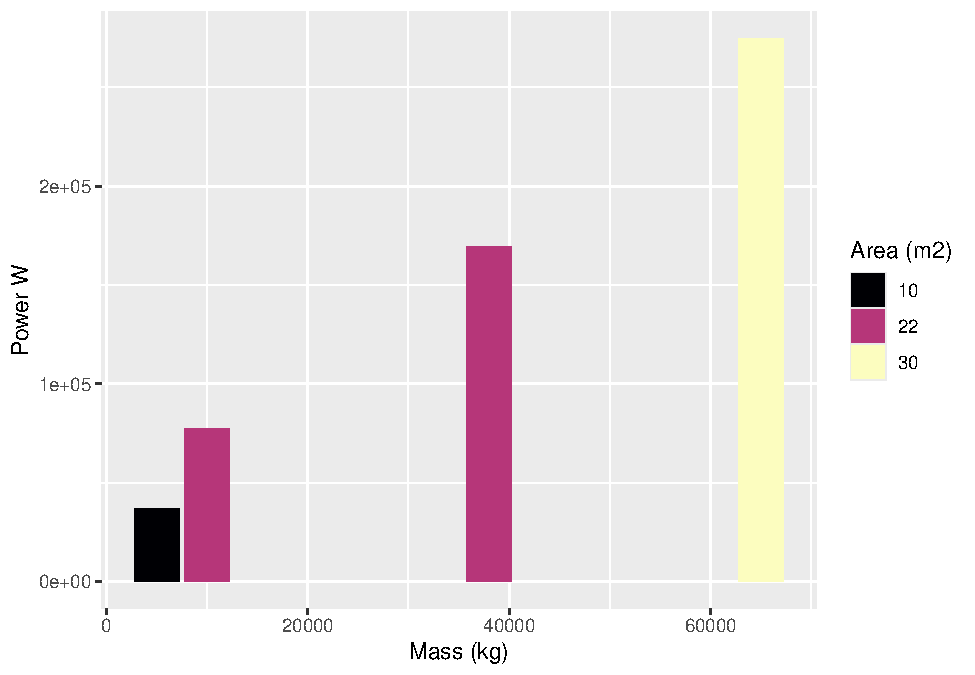
\includegraphics{looping_HW4_files/figure-latex/sampling2-1.pdf}

\section{Building a highway}\label{building-a-highway}

What could be the total power consumed if there are 200 cars on this
highway each hour, they are travelling at a range of speeds - mean is
80km/hr and speeds tend to be log-normally distributed)

How would the total power consumed vary by car So if all cars are car A;
OR all cars are car B; OR all cars are car C; OR all cars are car D

We will use \emph{sample} here to generate speeds for our 200 cars and
look at different ways to repeat power calculation for different cars

\begin{itemize}
\tightlist
\item
  repeating by hand
\item
  \emph{pmap} for repetition - a efficient way of looping in R
\item
  \emph{for} for repetition - a more standard way of looping available
  in many langugaes
\end{itemize}

\section{First lets do it `by hand'}\label{first-lets-do-it-by-hand}

\begin{Shaded}
\begin{Highlighting}[]
\CommentTok{\# what is I want to estimate average power use given  each car}

\NormalTok{possible\_cars}
\end{Highlighting}
\end{Shaded}

\begin{verbatim}
##   name  mass area     power
## 1    A 10000   22  77436.12
## 2    B 65000   30 274724.89
## 3    C 38000   22 169634.52
## 4    D  5000   10  36694.96
\end{verbatim}

\begin{Shaded}
\begin{Highlighting}[]
\CommentTok{\# use sample to generate a distribution of speeds}

\CommentTok{\# assume a log normal distribution of speeds with mean 100km/hr, and standard deviation that is 10 km/min {-}\textgreater{} convert into m/s (using *0.277)}

\CommentTok{\# recall our function needs speed in m/s not km/hr so we will also do a conversion}
\CommentTok{\# lets get a sample of a 200 speeds{-} we could also do this by actually measuring speeds}

\NormalTok{nsample }\OtherTok{=} \DecValTok{200}
\NormalTok{mean\_speed }\OtherTok{=} \FunctionTok{log}\NormalTok{(}\DecValTok{80}\SpecialCharTok{*}\FloatTok{0.277}\NormalTok{)}

\NormalTok{speeds }\OtherTok{=} \FunctionTok{rlnorm}\NormalTok{(}\AttributeTok{mean=}\NormalTok{mean\_speed, }\AttributeTok{sd=}\FunctionTok{log}\NormalTok{(}\DecValTok{10}\SpecialCharTok{*}\FloatTok{0.277}\NormalTok{), nsample)}
\FunctionTok{summary}\NormalTok{(speeds)}
\end{Highlighting}
\end{Shaded}

\begin{verbatim}
##    Min. 1st Qu.  Median    Mean 3rd Qu.    Max. 
##   2.304  11.712  24.993  44.610  48.989 503.145
\end{verbatim}

\begin{Shaded}
\begin{Highlighting}[]
\FunctionTok{plot}\NormalTok{(}\FunctionTok{density}\NormalTok{(speeds), }\AttributeTok{ylab=}\StringTok{"Distribution of Speeds in (m/s)"}\NormalTok{)}
\end{Highlighting}
\end{Shaded}

\includegraphics{looping_HW4_files/figure-latex/byhand-1.pdf}

\begin{Shaded}
\begin{Highlighting}[]
\CommentTok{\# how do we run each car for all speeds }

\CommentTok{\# first lets to it by hand for the first car {-} the first row in our possible cars matrix}
\NormalTok{possible\_cars[}\DecValTok{1}\NormalTok{,]}
\end{Highlighting}
\end{Shaded}

\begin{verbatim}
##   name  mass area    power
## 1    A 10000   22 77436.12
\end{verbatim}

\begin{Shaded}
\begin{Highlighting}[]
\CommentTok{\# we could do it by hand}
\CommentTok{\# aka: needing to put in individual car}
\NormalTok{powerA }\OtherTok{=} \FunctionTok{autopower}\NormalTok{(}\AttributeTok{V=}\NormalTok{speeds, }\AttributeTok{A =}\NormalTok{ possible\_cars}\SpecialCharTok{$}\NormalTok{area[}\DecValTok{1}\NormalTok{], }\AttributeTok{m=}\NormalTok{possible\_cars}\SpecialCharTok{$}\NormalTok{mass[}\DecValTok{1}\NormalTok{])}
\CommentTok{\# lets look at what we get}
\FunctionTok{summary}\NormalTok{(powerA)}
\end{Highlighting}
\end{Shaded}

\begin{verbatim}
##      Min.   1st Qu.    Median      Mean   3rd Qu.      Max. 
##      3436     23577     98562   7988587    537626 505139221
\end{verbatim}

\begin{Shaded}
\begin{Highlighting}[]
\CommentTok{\# next car (row 2)}
\NormalTok{powerB }\OtherTok{=} \FunctionTok{autopower}\NormalTok{(}\AttributeTok{V=}\NormalTok{speeds, }\AttributeTok{A =}\NormalTok{ possible\_cars}\SpecialCharTok{$}\NormalTok{area[}\DecValTok{2}\NormalTok{], }\AttributeTok{m=}\NormalTok{possible\_cars}\SpecialCharTok{$}\NormalTok{mass[}\DecValTok{2}\NormalTok{])}
\CommentTok{\# lets look at what we get}
\FunctionTok{summary}\NormalTok{(powerB)}
\end{Highlighting}
\end{Shaded}

\begin{verbatim}
##      Min.   1st Qu.    Median      Mean   3rd Qu.      Max. 
##     22084    120578    323109  11230353   1103018 692625183
\end{verbatim}

\begin{Shaded}
\begin{Highlighting}[]
\CommentTok{\# next car (row 3)}
\NormalTok{powerC }\OtherTok{=} \FunctionTok{autopower}\NormalTok{(}\AttributeTok{V=}\NormalTok{speeds, }\AttributeTok{A =}\NormalTok{ possible\_cars}\SpecialCharTok{$}\NormalTok{area[}\DecValTok{3}\NormalTok{], }\AttributeTok{m=}\NormalTok{possible\_cars}\SpecialCharTok{$}\NormalTok{mass[}\DecValTok{3}\NormalTok{])}
\CommentTok{\# lets look at what we get}
\FunctionTok{summary}\NormalTok{(powerC)}
\end{Highlighting}
\end{Shaded}

\begin{verbatim}
##      Min.   1st Qu.    Median      Mean   3rd Qu.      Max. 
##     12920     71782    201432   8172201    739266 507210165
\end{verbatim}

\begin{Shaded}
\begin{Highlighting}[]
\CommentTok{\# next car (row 4)}
\NormalTok{powerD }\OtherTok{=} \FunctionTok{autopower}\NormalTok{(}\AttributeTok{V=}\NormalTok{speeds, }\AttributeTok{A =}\NormalTok{ possible\_cars}\SpecialCharTok{$}\NormalTok{area[}\DecValTok{4}\NormalTok{], }\AttributeTok{m=}\NormalTok{possible\_cars}\SpecialCharTok{$}\NormalTok{mass[}\DecValTok{4}\NormalTok{])}
\CommentTok{\# lets look at what we get}
\FunctionTok{summary}\NormalTok{(powerD)}
\end{Highlighting}
\end{Shaded}

\begin{verbatim}
##      Min.   1st Qu.    Median      Mean   3rd Qu.      Max. 
##      1716     11499     46471   3634157    247649 229642356
\end{verbatim}

\begin{Shaded}
\begin{Highlighting}[]
\CommentTok{\# we could put this together}
\NormalTok{powerall1 }\OtherTok{=} \FunctionTok{cbind.data.frame}\NormalTok{(powerA, powerB, powerC, powerD)}
\FunctionTok{colnames}\NormalTok{(powerall1)}\OtherTok{=}\NormalTok{possible\_cars}\SpecialCharTok{$}\NormalTok{name}


\CommentTok{\# for plotting sometimes its useful to turn columns in to rows {-} we can use an R function}
\CommentTok{\# called pivot\_longer (part of the tidyverse package) to do this}
\CommentTok{\# compare powerall1 and powerallr1 to see what pivot\_longer does}
\NormalTok{powerallr1 }\OtherTok{=}\NormalTok{ powerall1 }\SpecialCharTok{|\textgreater{}} \FunctionTok{pivot\_longer}\NormalTok{(}\AttributeTok{cols=}\FunctionTok{everything}\NormalTok{(), }\AttributeTok{names\_to=}\StringTok{"car"}\NormalTok{, }\AttributeTok{values\_to=}\StringTok{"power"}\NormalTok{)}
\FunctionTok{head}\NormalTok{(powerallr1)}
\end{Highlighting}
\end{Shaded}

\begin{verbatim}
## # A tibble: 6 x 2
##   car      power
##   <chr>    <dbl>
## 1 A       14905.
## 2 B       84432.
## 3 C       49852.
## 4 D        7342.
## 5 A     3864537.
## 6 B     6009334.
\end{verbatim}

\begin{Shaded}
\begin{Highlighting}[]
\NormalTok{powerall1}
\end{Highlighting}
\end{Shaded}

\begin{verbatim}
##                A            B            C            D
## 1   1.490483e+04     84431.93     49851.75 7.342244e+03
## 2   3.864537e+06   6009333.53   4267668.33 1.763152e+06
## 3   2.388507e+05    598046.00    387312.42 1.109786e+05
## 4   2.638612e+06   4246888.79   2992284.03 1.205110e+06
## 5   9.389988e+04    312722.55    194573.50 4.431608e+04
## 6   2.288320e+05    579846.23    374819.96 1.063845e+05
## 7   5.025523e+06   7661820.37   5466445.12 2.291486e+06
## 8   3.065684e+04    145927.55     87417.57 1.485637e+04
## 9   3.867271e+04    171738.14    103544.94 1.863163e+04
## 10  5.328008e+03     33753.84     19767.69 2.656232e+03
## 11  2.293510e+04    118123.83     70279.16 1.119362e+04
## 12  1.033947e+04     62009.85     36457.09 5.123745e+03
## 13  1.075545e+04     64175.92     37744.64 5.326976e+03
## 14  2.165161e+04    113125.69     67225.13 1.058147e+04
## 15  3.094862e+05    723026.23    473570.93 1.433392e+05
## 16  2.292230e+04    118074.58     70249.03 1.118752e+04
## 17  1.064422e+06   1924293.75   1322165.89 4.880125e+05
## 18  1.116576e+06   2003473.28   1378713.87 5.117902e+05
## 19  1.668799e+04     92465.34     54688.64 8.202342e+03
## 20  2.215378e+05    566505.51    365675.53 1.030389e+05
## 21  3.852934e+05    852385.30    563543.75 1.780271e+05
## 22  2.860124e+06   4567194.41   3223741.23 1.305959e+06
## 23  1.820938e+06   3053776.73   2132033.99 8.327492e+05
## 24  4.724644e+04    196999.81    119516.24 2.264887e+04
## 25  1.135708e+04     67262.48     39581.63 5.620498e+03
## 26  1.336334e+04     77178.63     45502.13 6.595979e+03
## 27  5.715001e+04    224052.29    136805.06 2.727038e+04
## 28  1.322236e+05    394578.31    249031.05 6.199787e+04
## 29  5.733386e+03     36188.06     21198.70 2.857145e+03
## 30  8.959837e+03     54633.18     32081.76 4.448009e+03
## 31  3.455116e+04    158783.42     95425.15 1.669329e+04
## 32  1.064476e+05    340371.08    212865.83 5.011285e+04
## 33  9.551083e+05   1757410.50   1203138.30 4.381666e+05
## 34  2.844932e+04    138327.02     82707.74 1.381233e+04
## 35  3.597961e+04    163342.92     98277.28 1.736569e+04
## 36  3.536723e+05    798908.44    526276.60 1.635621e+05
## 37  5.301588e+04    212992.08    129714.80 2.534324e+04
## 38  1.252239e+04     73090.59     43057.78 6.187698e+03
## 39  6.034286e+04    232396.21    142173.01 2.875699e+04
## 40  8.007698e+04    280975.94    173719.91 3.791881e+04
## 41  1.351081e+04     77885.72     45925.43 6.667488e+03
## 42  1.550360e+05    440395.90    279862.23 7.249732e+04
## 43  5.352137e+03     33899.43     19853.24 2.668197e+03
## 44  3.435820e+03     22083.96     12920.45 1.715708e+03
## 45  4.226579e+06   6525997.47   4642232.29 1.927920e+06
## 46  1.276739e+06   2245122.46   1551548.46 5.847971e+05
## 47  5.482902e+05   1120233.86    751387.79 2.525198e+05
## 48  3.192225e+06   5045700.40   3569820.10 1.457141e+06
## 49  2.293573e+04    118126.26     70280.65 1.119392e+04
## 50  2.669505e+04    132102.14     78864.14 1.298101e+04
## 51  4.186349e+05    908143.22    602495.87 1.932733e+05
## 52  9.701981e+03     58638.56     34455.69 4.811837e+03
## 53  3.878627e+05    856703.78    566557.27 1.792021e+05
## 54  1.288337e+04     74857.17     44113.45 6.363059e+03
## 55  1.929180e+06   3212936.18   2246575.98 8.820525e+05
## 56  1.684156e+04     93140.58     55096.15 8.276273e+03
## 57  1.726110e+04     94972.31     56202.35 8.478116e+03
## 58  1.910117e+05    509735.73    326894.35 8.902940e+04
## 59  5.617381e+03     35494.02     20790.58 2.799673e+03
## 60  1.510953e+05    432599.39    274600.76 7.068463e+04
## 61  3.235327e+06   5107668.84   3614662.64 1.476761e+06
## 62  2.888173e+05    686983.96    448618.70 1.338748e+05
## 63  1.009290e+04     60713.38     35687.06 5.003169e+03
## 64  2.585287e+04    129050.34     76984.37 1.258136e+04
## 65  9.800788e+04    321883.42    200621.66 4.621485e+04
## 66  3.698698e+06   5772180.42   4095827.88 1.687673e+06
## 67  7.307345e+06  10883051.28   7808043.86 3.329649e+06
## 68  1.723151e+04     94843.72     56124.66 8.463885e+03
## 69  2.283891e+04    117753.55     70052.63 1.114778e+04
## 70  5.051392e+08 692625183.43 507210165.44 2.296424e+08
## 71  3.105235e+05    724825.24    474817.85 1.438142e+05
## 72  8.727032e+05   1630657.24   1112892.74 4.005825e+05
## 73  3.101639e+04    147142.74     88172.28 1.502621e+04
## 74  4.998769e+04    204685.81    124409.64 2.392983e+04
## 75  3.680715e+05    823337.61    543289.12 1.701497e+05
## 76  5.163302e+05   1068546.30    715009.10 2.379209e+05
## 77  1.124220e+05    353214.98    221400.72 5.287006e+04
## 78  9.945144e+06  14580996.91  10500872.54 4.529542e+06
## 79  1.382104e+04     79363.93     46810.87 6.817842e+03
## 80  4.792744e+04    198924.91    120740.44 2.296723e+04
## 81  3.615104e+04    163884.96     98616.76 1.744635e+04
## 82  6.215141e+04    237052.72    145175.56 2.959844e+04
## 83  3.234009e+05    747083.50    490256.36 1.497091e+05
## 84  2.473977e+05    613466.05    397911.88 1.148969e+05
## 85  3.379438e+07  47621638.84  34633008.56 1.537470e+07
## 86  2.880699e+05    685673.31    447712.41 1.335325e+05
## 87  7.927267e+04    279079.10    172479.47 3.754613e+04
## 88  2.456401e+05    610302.72    395736.38 1.140912e+05
## 89  3.426188e+06   5381738.74   3813049.16 1.563638e+06
## 90  1.144707e+08 158410634.02 115732263.44 5.205262e+07
## 91  6.218479e+06   9349319.37   6692513.06 2.834277e+06
## 92  5.036755e+03     31989.76     18731.28 2.511748e+03
## 93  2.473913e+06   4008049.83   2819817.17 1.130121e+06
## 94  4.117685e+05    896708.71    594500.37 1.901339e+05
## 95  2.425235e+06   3937336.24   2768776.23 1.107956e+06
## 96  1.649997e+05    459914.83    293059.69 7.707876e+04
## 97  4.017255e+04    176308.80    106421.47 1.933572e+04
## 98  1.601075e+05    450364.48    286597.97 7.482956e+04
## 99  2.272004e+04    117295.02     69772.16 1.109112e+04
## 100 3.733128e+05    832196.98    549463.76 1.725472e+05
## 101 5.418375e+04    216147.75    131734.78 2.588792e+04
## 102 9.634689e+03     58278.99     34242.40 4.778880e+03
## 103 2.017083e+04    107196.31     63612.81 9.873786e+03
## 104 1.266485e+04     73789.94     43475.58 6.256926e+03
## 105 2.569332e+04    128467.30     76625.59 1.250561e+04
## 106 1.100425e+04     65458.91     38507.89 5.448418e+03
## 107 7.434794e+05   1429873.00    970275.03 3.416269e+05
## 108 2.457338e+08 338078397.10 247362022.42 1.117236e+08
## 109 2.360414e+04    120680.65     71844.67 1.151228e+04
## 110 2.923915e+05    693244.57    452948.84 1.355117e+05
## 111 9.542605e+03     57785.78     33949.91 4.733770e+03
## 112 4.588355e+08 629363855.72 460841097.16 2.085942e+08
## 113 1.349893e+04     77828.86     45891.39 6.661729e+03
## 114 2.653600e+05    645579.84    420027.94 1.231290e+05
## 115 7.111451e+05   1379177.05    934340.83 3.268711e+05
## 116 3.588995e+06   5615118.43   3982054.31 1.637742e+06
## 117 2.455661e+04    124266.57     74043.91 1.196546e+04
## 118 1.916704e+04    103069.59     61105.58 9.393111e+03
## 119 8.636651e+03     52861.40     31032.96 4.289327e+03
## 120 1.446344e+04     82385.58     48622.93 7.128828e+03
## 121 2.412385e+05    602363.48    390278.82 1.120733e+05
## 122 4.231452e+05    915641.29    607740.83 1.953354e+05
## 123 3.307492e+04    153986.77     92431.48 1.599763e+04
## 124 2.229538e+05    569101.50    367454.09 1.036884e+05
## 125 7.759796e+05   1480632.14   1006286.26 3.564567e+05
## 126 1.958602e+05    518863.56    333114.53 9.125554e+04
## 127 1.193273e+05    367836.25    231143.40 5.605488e+04
## 128 1.249294e+05    379537.90    238960.07 5.863725e+04
## 129 6.916208e+04    254676.85    156582.25 3.285647e+04
## 130 3.285237e+04    153255.84     91975.92 1.589269e+04
## 131 3.620371e+04    164051.27     98720.94 1.747112e+04
## 132 1.332884e+06   2329358.13   1611876.96 6.103855e+05
## 133 2.349661e+04    120271.89     71594.25 1.146108e+04
## 134 1.442443e+04     82203.58     48513.71 7.109957e+03
## 135 4.560178e+04    192305.49    116535.13 2.187960e+04
## 136 3.483650e+05    789869.64    519987.20 1.611338e+05
## 137 2.033893e+05    532950.46    342726.01 9.471166e+04
## 138 1.015363e+06   1849561.74   1268836.67 4.656437e+05
## 139 3.445702e+04    158480.15     95235.67 1.664895e+04
## 140 1.693342e+04     93543.24     55339.23 8.320482e+03
## 141 7.626042e+04    271920.21    167803.87 3.614992e+04
## 142 5.859007e+03     36937.30     21639.37 2.919360e+03
## 143 4.892070e+04    201713.89    122515.71 2.343140e+04
## 144 7.185768e+05   1390847.09    942609.80 3.302627e+05
## 145 1.073211e+06   1937655.45   1331705.31 4.920196e+05
## 146 3.479983e+04    159582.78     95924.73 1.681039e+04
## 147 2.954613e+04    142134.14     85064.61 1.433133e+04
## 148 2.056315e+06   3399326.16   2380810.85 9.399564e+05
## 149 1.623526e+06   2762236.55   1922442.70 7.428189e+05
## 150 1.848108e+05    497993.84    318902.08 8.618173e+04
## 151 1.491140e+05    428662.10    271945.94 6.977311e+04
## 152 4.654970e+06   7135690.94   5084537.07 2.122869e+06
## 153 5.340710e+05   1097279.59    735225.51 2.460251e+05
## 154 1.825655e+04     99245.93     58787.52 8.956402e+03
## 155 8.938395e+04    302516.09    187850.67 4.222755e+04
## 156 2.652493e+04    131489.10     78486.29 1.290031e+04
## 157 2.138021e+05    552268.63    355929.28 9.949003e+04
## 158 3.871129e+04    171856.60    103619.41 1.864974e+04
## 159 1.590046e+05    448202.57    285136.38 7.432240e+04
## 160 1.981176e+05    523097.92    336002.13 9.229182e+04
## 161 6.081223e+04    233609.39    142954.81 2.897541e+04
## 162 7.378945e+05   1421131.04    964076.22 3.390784e+05
## 163 1.825043e+05    493605.91    315918.12 8.512230e+04
## 164 1.903992e+06   3175939.69   2219943.77 8.705799e+05
## 165 1.400948e+06   2431186.25   1684854.65 6.414036e+05
## 166 1.305076e+04     75670.30     44599.67 6.444321e+03
## 167 2.174797e+07  30983154.77  22471268.54 9.897181e+06
## 168 8.341068e+04    288775.48    178827.25 3.946292e+04
## 169 1.030108e+04     61808.63     36337.55 5.104978e+03
## 170 8.257329e+04    286825.55    177549.37 3.907513e+04
## 171 2.245477e+04    116267.99     69144.21 1.096466e+04
## 172 9.614618e+04    317745.78    197888.31 4.535446e+04
## 173 1.547144e+04     87024.31     51410.34 7.615895e+03
## 174 8.111343e+03     49945.53     29308.61 4.031086e+03
## 175 1.727949e+05    475007.02    303287.48 8.066153e+04
## 176 4.665857e+05    987369.98    657990.94 2.151916e+05
## 177 5.988554e+05   1201364.36    808591.59 2.756118e+05
## 178 1.309900e+05    392049.38    247335.86 6.142965e+04
## 179 3.323906e+04    154524.54     92766.76 1.607502e+04
## 180 3.350921e+04    155407.15     93317.23 1.620237e+04
## 181 8.635916e+05   1616585.51   1102883.41 3.964263e+05
## 182 7.335122e+05   1414267.37    959209.95 3.370786e+05
## 183 3.218694e+04    151057.55     90606.78 1.557880e+04
## 184 3.224409e+05    745428.88    489108.02 1.492697e+05
## 185 9.911568e+04    324334.86    202242.32 4.672672e+04
## 186 2.062978e+05    538364.87    346423.99 9.604648e+04
## 187 3.058490e+06   4853236.18   3430580.04 1.396263e+06
## 188 4.723376e+04    196963.86    119493.39 2.264294e+04
## 189 2.401666e+07  34121803.86  24764481.06 1.092881e+07
## 190 5.659121e+04    222574.86    135856.25 2.701005e+04
## 191 2.319024e+07  32978822.33  23929313.05 1.055302e+07
## 192 6.971261e+03     43463.03     25482.20 3.469257e+03
## 193 1.041182e+04     62388.49     36682.07 5.159109e+03
## 194 6.073421e+04    233407.97    142824.98 2.893910e+04
## 195 4.871526e+04    201138.84    122149.51 2.333541e+04
## 196 1.493900e+05    429211.26    272316.13 6.990008e+04
## 197 3.813510e+04    170082.11    102504.21 1.837909e+04
## 198 5.509051e+07  76935471.69  56078316.95 2.505718e+07
## 199 6.478291e+03     40594.95     23792.20 3.225748e+03
## 200 2.166097e+06   3559841.95   2496487.42 9.899530e+05
\end{verbatim}

\begin{Shaded}
\begin{Highlighting}[]
\CommentTok{\# note: powerallr1 has 800 values in column, 200 observations for each car }
\CommentTok{\# \textgreater{} (nsample = 200)}


\CommentTok{\# quick visualization}
\CommentTok{\# lets save it so that we can compare}
\NormalTok{method1\_plot }\OtherTok{=} \FunctionTok{ggplot}\NormalTok{(powerallr1, }\FunctionTok{aes}\NormalTok{(car,power, }\AttributeTok{fill=}\NormalTok{car))}\SpecialCharTok{+}\FunctionTok{geom\_boxplot}\NormalTok{()}\SpecialCharTok{+}\FunctionTok{ggtitle}\NormalTok{(}\StringTok{"By Hand"}\NormalTok{)}\SpecialCharTok{+}
  \FunctionTok{ylim}\NormalTok{(}\DecValTok{0}\NormalTok{,}\DecValTok{2000000}\NormalTok{)}
\NormalTok{method1\_plot}
\end{Highlighting}
\end{Shaded}

\begin{verbatim}
## Warning: Removed 109 rows containing non-finite outside the scale range
## (`stat_boxplot()`).
\end{verbatim}

\includegraphics{looping_HW4_files/figure-latex/byhand-2.pdf}

\section{Second using R built in
tools}\label{second-using-r-built-in-tools}

Doing this by hand would be hard if we had many different cars - can we
automate?

YES

first lets try \emph{pmap}

\emph{pmap} is available in the \emph{purr} library

\emph{mapply} is another R option

\begin{Shaded}
\begin{Highlighting}[]
\CommentTok{\# the first part, generating speeds is the same}
\CommentTok{\# what is I want to estimate average power use given  each car}

\NormalTok{possible\_cars}
\end{Highlighting}
\end{Shaded}

\begin{verbatim}
##   name  mass area     power
## 1    A 10000   22  77436.12
## 2    B 65000   30 274724.89
## 3    C 38000   22 169634.52
## 4    D  5000   10  36694.96
\end{verbatim}

\begin{Shaded}
\begin{Highlighting}[]
\CommentTok{\# the first part is the same as above}
\CommentTok{\# use sample to generate a distribution of speeds}

\CommentTok{\# assume a log normal distribution of speeds with mean 80km/hr}
\CommentTok{\# recall our function needs speed in m/s not km/hr so we will also do a conversion}
\CommentTok{\# lets get a sample of a 200 speeds{-} we could also do this by actually measuring speeds}

\NormalTok{nsample }\OtherTok{=} \DecValTok{200}
\NormalTok{mean\_speed }\OtherTok{=} \FunctionTok{log}\NormalTok{(}\DecValTok{80}\SpecialCharTok{*}\FloatTok{0.277}\NormalTok{)}

\NormalTok{speeds }\OtherTok{=} \FunctionTok{rlnorm}\NormalTok{(}\AttributeTok{mean=}\NormalTok{mean\_speed, }\AttributeTok{sd=}\FunctionTok{log}\NormalTok{(}\DecValTok{10}\SpecialCharTok{*}\FloatTok{0.277}\NormalTok{), nsample)}
\FunctionTok{summary}\NormalTok{(speeds)}
\end{Highlighting}
\end{Shaded}

\begin{verbatim}
##    Min. 1st Qu.  Median    Mean 3rd Qu.    Max. 
##   1.871  11.381  24.320  43.291  52.135 415.223
\end{verbatim}

\begin{Shaded}
\begin{Highlighting}[]
\FunctionTok{plot}\NormalTok{(}\FunctionTok{density}\NormalTok{(speeds), }\AttributeTok{ylab=}\StringTok{"Distribution of Speeds in (m/s)"}\NormalTok{)}
\end{Highlighting}
\end{Shaded}

\includegraphics{looping_HW4_files/figure-latex/withpmap-1.pdf}

\begin{Shaded}
\begin{Highlighting}[]
\CommentTok{\# how do we run each car for all speeds }
\CommentTok{\# pmap runs a function for each value in a list of parameters, with other parameters set for each iteration}


\NormalTok{powerall2 }\OtherTok{=} \FunctionTok{pmap}\NormalTok{(}\FunctionTok{list}\NormalTok{(}\AttributeTok{A =}\NormalTok{ possible\_cars}\SpecialCharTok{$}\NormalTok{area, }\AttributeTok{m=}\NormalTok{possible\_cars}\SpecialCharTok{$}\NormalTok{mass), autopower, }\AttributeTok{V=}\NormalTok{speeds)}

\CommentTok{\# lets turn to a data frame for easier graphing}
\CommentTok{\# we can add column names}
\NormalTok{powerall2 }\OtherTok{=} \FunctionTok{as.data.frame}\NormalTok{(powerall2, }\AttributeTok{col.names=}\NormalTok{possible\_cars}\SpecialCharTok{$}\NormalTok{name)}

\CommentTok{\# apply family of functions does this to {-} FYI}
\CommentTok{\# what mapply does is run the function for each row in parameters listed, using values for other parameters listed in MoreArgs EACH time {-} a column for row in parameter list is returned}
\NormalTok{powerall2b }\OtherTok{=} \FunctionTok{mapply}\NormalTok{(}\AttributeTok{FUN=}\NormalTok{autopower, }\AttributeTok{A =}\NormalTok{ possible\_cars}\SpecialCharTok{$}\NormalTok{area, }\AttributeTok{m=}\NormalTok{possible\_cars}\SpecialCharTok{$}\NormalTok{mass, }\AttributeTok{MoreArgs =} \FunctionTok{list}\NormalTok{(}\AttributeTok{V=}\NormalTok{speeds)  )}
\CommentTok{\# we can add column names}
\FunctionTok{colnames}\NormalTok{(powerall2b)}\OtherTok{=}\NormalTok{possible\_cars}\SpecialCharTok{$}\NormalTok{name}

\FunctionTok{head}\NormalTok{(powerall2b)}
\end{Highlighting}
\end{Shaded}

\begin{verbatim}
##                A          B          C          D
## [1,] 1505694.240 2587325.26 1796852.82 689133.073
## [2,]    5417.280   34292.03   20083.99   2700.496
## [3,]   12556.586   73258.73   43158.22   6204.319
## [4,]    2776.261   17912.48   10477.17   1386.951
## [5,]   88952.012  301531.98  187203.35  42027.722
## [6,]   73475.576  265220.67  163437.04  34858.402
\end{verbatim}

\begin{Shaded}
\begin{Highlighting}[]
\FunctionTok{head}\NormalTok{(powerall2)}
\end{Highlighting}
\end{Shaded}

\begin{verbatim}
##             A          B          C          D
## 1 1505694.240 2587325.26 1796852.82 689133.073
## 2    5417.280   34292.03   20083.99   2700.496
## 3   12556.586   73258.73   43158.22   6204.319
## 4    2776.261   17912.48   10477.17   1386.951
## 5   88952.012  301531.98  187203.35  42027.722
## 6   73475.576  265220.67  163437.04  34858.402
\end{verbatim}

\begin{Shaded}
\begin{Highlighting}[]
\CommentTok{\# for plotting sometimes its useful to turn columns in to rows}
\NormalTok{powerallr2 }\OtherTok{=}\NormalTok{ powerall2 }\SpecialCharTok{|\textgreater{}} \FunctionTok{pivot\_longer}\NormalTok{(}\AttributeTok{cols=}\FunctionTok{everything}\NormalTok{(), }\AttributeTok{names\_to=}\StringTok{"car"}\NormalTok{, }\AttributeTok{values\_to=}\StringTok{"power"}\NormalTok{)}
\FunctionTok{head}\NormalTok{(powerallr2)}
\end{Highlighting}
\end{Shaded}

\begin{verbatim}
## # A tibble: 6 x 2
##   car      power
##   <chr>    <dbl>
## 1 A     1505694.
## 2 B     2587325.
## 3 C     1796853.
## 4 D      689133.
## 5 A        5417.
## 6 B       34292.
\end{verbatim}

\begin{Shaded}
\begin{Highlighting}[]
\CommentTok{\# quick visualization}

\NormalTok{method2\_plot }\OtherTok{=} \FunctionTok{ggplot}\NormalTok{(powerallr2, }\FunctionTok{aes}\NormalTok{(car,power, }\AttributeTok{fill=}\NormalTok{car))}\SpecialCharTok{+}\FunctionTok{geom\_boxplot}\NormalTok{()}\SpecialCharTok{+}\FunctionTok{ggtitle}\NormalTok{(}\StringTok{"pmap"}\NormalTok{)}
\NormalTok{method2\_plot}\SpecialCharTok{+}
  \FunctionTok{ylim}\NormalTok{(}\DecValTok{0}\NormalTok{,}\DecValTok{2000000}\NormalTok{)}
\end{Highlighting}
\end{Shaded}

\begin{verbatim}
## Warning: Removed 115 rows containing non-finite outside the scale range
## (`stat_boxplot()`).
\end{verbatim}

\includegraphics{looping_HW4_files/figure-latex/withpmap-2.pdf}

\begin{Shaded}
\begin{Highlighting}[]
\NormalTok{method2\_plot}
\end{Highlighting}
\end{Shaded}

\includegraphics{looping_HW4_files/figure-latex/withpmap-3.pdf}

\begin{Shaded}
\begin{Highlighting}[]
\CommentTok{\# put plots side by side}
\CommentTok{\# to confirm that they look similar}
\FunctionTok{ggarrange}\NormalTok{(method1\_plot, method2\_plot)}
\end{Highlighting}
\end{Shaded}

\begin{verbatim}
## Warning: Removed 109 rows containing non-finite outside the scale range
## (`stat_boxplot()`).
\end{verbatim}

\includegraphics{looping_HW4_files/figure-latex/withpmap-4.pdf}

\begin{Shaded}
\begin{Highlighting}[]
\CommentTok{\# compare values}
\FunctionTok{head}\NormalTok{(powerallr2)}
\end{Highlighting}
\end{Shaded}

\begin{verbatim}
## # A tibble: 6 x 2
##   car      power
##   <chr>    <dbl>
## 1 A     1505694.
## 2 B     2587325.
## 3 C     1796853.
## 4 D      689133.
## 5 A        5417.
## 6 B       34292.
\end{verbatim}

\begin{Shaded}
\begin{Highlighting}[]
\FunctionTok{head}\NormalTok{(powerallr1)}
\end{Highlighting}
\end{Shaded}

\begin{verbatim}
## # A tibble: 6 x 2
##   car      power
##   <chr>    <dbl>
## 1 A       14905.
## 2 B       84432.
## 3 C       49852.
## 4 D        7342.
## 5 A     3864537.
## 6 B     6009334.
\end{verbatim}

\begin{Shaded}
\begin{Highlighting}[]
\CommentTok{\# not exactly the same {-} why?}
\CommentTok{\# recall that we sample speeds!}
\end{Highlighting}
\end{Shaded}

\section{\texorpdfstring{Third - classic looping
\emph{for}}{Third - classic looping for}}\label{third---classic-looping-for}

\emph{pmap} works quickly but it is unique to R Other programming
language (and R) use what are called loops - where repetition is more
explicit

Lets do this one more time using a \emph{for} loop

\begin{Shaded}
\begin{Highlighting}[]
\CommentTok{\# the first part, generating speeds is the same}
\CommentTok{\# proceed with estimating average power use given  each car}

\NormalTok{possible\_cars}
\end{Highlighting}
\end{Shaded}

\begin{verbatim}
##   name  mass area     power
## 1    A 10000   22  77436.12
## 2    B 65000   30 274724.89
## 3    C 38000   22 169634.52
## 4    D  5000   10  36694.96
\end{verbatim}

\begin{Shaded}
\begin{Highlighting}[]
\CommentTok{\# use sample to generate a distribution of speeds}

\CommentTok{\# assume a log normal distribution of speeds with mean 80km/hr}
\CommentTok{\# recall our function needs speed in m/s not km/hr so we will also do a conversion}
\CommentTok{\# lets get a sample of a 200 speeds{-} we could also do this by actually measuring speeds}

\NormalTok{nsample }\OtherTok{=} \DecValTok{200}
\NormalTok{mean\_speed }\OtherTok{=} \FunctionTok{log}\NormalTok{(}\DecValTok{80}\SpecialCharTok{*}\FloatTok{0.277}\NormalTok{)}

\NormalTok{speeds }\OtherTok{=} \FunctionTok{rlnorm}\NormalTok{(}\AttributeTok{mean=}\NormalTok{mean\_speed, }\AttributeTok{sd=}\FunctionTok{log}\NormalTok{(}\DecValTok{10}\SpecialCharTok{*}\FloatTok{0.277}\NormalTok{), nsample)}
\FunctionTok{summary}\NormalTok{(speeds)}
\end{Highlighting}
\end{Shaded}

\begin{verbatim}
##    Min. 1st Qu.  Median    Mean 3rd Qu.    Max. 
##   1.277   9.658  19.608  34.698  38.351 303.360
\end{verbatim}

\begin{Shaded}
\begin{Highlighting}[]
\FunctionTok{plot}\NormalTok{(}\FunctionTok{density}\NormalTok{(speeds), }\AttributeTok{ylab=}\StringTok{"Distribution of Speeds in (m/s)"}\NormalTok{)}
\end{Highlighting}
\end{Shaded}

\includegraphics{looping_HW4_files/figure-latex/withforloop-1.pdf}

\begin{Shaded}
\begin{Highlighting}[]
\CommentTok{\# how do we run each car for all speeds }
\CommentTok{\# we use a for loop to cycle through}
\CommentTok{\# we need to create a data frame to store results {-} as above}
\CommentTok{\# one column for each car and one row for each speed}

\NormalTok{powerall3 }\OtherTok{=} \FunctionTok{as.data.frame}\NormalTok{(}\FunctionTok{matrix}\NormalTok{(}\AttributeTok{nrow=}\FunctionTok{length}\NormalTok{(speeds), }\AttributeTok{ncol=}\FunctionTok{nrow}\NormalTok{(possible\_cars)))}
\CommentTok{\# because we don\textquotesingle{}t initialize it {-} values are NA}
\FunctionTok{head}\NormalTok{(powerall3)}
\end{Highlighting}
\end{Shaded}

\begin{verbatim}
##   V1 V2 V3 V4
## 1 NA NA NA NA
## 2 NA NA NA NA
## 3 NA NA NA NA
## 4 NA NA NA NA
## 5 NA NA NA NA
## 6 NA NA NA NA
\end{verbatim}

\begin{Shaded}
\begin{Highlighting}[]
\CommentTok{\# how many cars area there}
\FunctionTok{nrow}\NormalTok{(possible\_cars)}
\end{Highlighting}
\end{Shaded}

\begin{verbatim}
## [1] 4
\end{verbatim}

\begin{Shaded}
\begin{Highlighting}[]
\CommentTok{\# for loops use an index {-} in this case "i" but you could use anything {-} it repeats}
\CommentTok{\# anything between the \{\} for each values of i between 1 and nrow(possible\_car) (which is 3 in our case)}


\CommentTok{\# index in to a matrix (like powerall3) is by row and column powerall3[2,5] is 2nd row and 5th column}
\ControlFlowTok{for}\NormalTok{ (i }\ControlFlowTok{in} \DecValTok{1}\SpecialCharTok{:}\FunctionTok{nrow}\NormalTok{(possible\_cars)) \{}
\NormalTok{  powerall3[,i] }\OtherTok{=} \FunctionTok{autopower}\NormalTok{(}\AttributeTok{A=}\NormalTok{possible\_cars}\SpecialCharTok{$}\NormalTok{area[i], }\AttributeTok{m=}\NormalTok{possible\_cars}\SpecialCharTok{$}\NormalTok{mass[i], }\AttributeTok{V=}\NormalTok{speeds)}
\NormalTok{\}}

\CommentTok{\# now it looks like above}
\FunctionTok{head}\NormalTok{(powerall3)}
\end{Highlighting}
\end{Shaded}

\begin{verbatim}
##            V1         V2         V3          V4
## 1   58350.879  227209.69  138834.44   27829.678
## 2 4402646.172 6776780.98 4824127.86 2008045.040
## 3   21597.773  112913.27   67095.51   10555.769
## 4  102872.013  332590.38  207706.69   48461.867
## 5    5241.897   33233.58   19461.98    2613.526
## 6   37990.445  169634.89  102223.29   18311.125
\end{verbatim}

\begin{Shaded}
\begin{Highlighting}[]
\CommentTok{\# we can add column names}
\FunctionTok{colnames}\NormalTok{(powerall3)}\OtherTok{=}\NormalTok{possible\_cars}\SpecialCharTok{$}\NormalTok{name}

\CommentTok{\# plotting is the same as above}

\CommentTok{\# for plotting sometimes its useful to turn columns in to rows}
\NormalTok{powerallr3 }\OtherTok{=}\NormalTok{ powerall3 }\SpecialCharTok{|\textgreater{}} \FunctionTok{pivot\_longer}\NormalTok{(}\AttributeTok{cols=}\FunctionTok{everything}\NormalTok{(), }\AttributeTok{names\_to=}\StringTok{"car"}\NormalTok{, }\AttributeTok{values\_to=}\StringTok{"power"}\NormalTok{)}
\FunctionTok{head}\NormalTok{(powerallr3)}
\end{Highlighting}
\end{Shaded}

\begin{verbatim}
## # A tibble: 6 x 2
##   car      power
##   <chr>    <dbl>
## 1 A       58351.
## 2 B      227210.
## 3 C      138834.
## 4 D       27830.
## 5 A     4402646.
## 6 B     6776781.
\end{verbatim}

\begin{Shaded}
\begin{Highlighting}[]
\CommentTok{\# quick visualization}
\NormalTok{method3\_plot }\OtherTok{=} \FunctionTok{ggplot}\NormalTok{(powerallr3, }\FunctionTok{aes}\NormalTok{(car,power, }\AttributeTok{fill=}\NormalTok{car))}\SpecialCharTok{+}\FunctionTok{geom\_boxplot}\NormalTok{()}\SpecialCharTok{+}\FunctionTok{ggtitle}\NormalTok{(}\StringTok{"For Loop"}\NormalTok{)}\SpecialCharTok{+}
    \FunctionTok{ylim}\NormalTok{(}\DecValTok{0}\NormalTok{,}\DecValTok{2000000}\NormalTok{)}

\FunctionTok{ggarrange}\NormalTok{(method1\_plot, method2\_plot, method3\_plot, }\AttributeTok{nrow=}\DecValTok{3}\NormalTok{)}
\end{Highlighting}
\end{Shaded}

\begin{verbatim}
## Warning: Removed 109 rows containing non-finite outside the scale range
## (`stat_boxplot()`).
\end{verbatim}

\begin{verbatim}
## Warning: Removed 95 rows containing non-finite outside the scale range
## (`stat_boxplot()`).
\end{verbatim}

\includegraphics{looping_HW4_files/figure-latex/withforloop-2.pdf}

\begin{Shaded}
\begin{Highlighting}[]
\NormalTok{powerall1 }\SpecialCharTok{|\textgreater{}} \FunctionTok{map}\NormalTok{(mean)}
\end{Highlighting}
\end{Shaded}

\begin{verbatim}
## $A
## [1] 7988587
## 
## $B
## [1] 11230353
## 
## $C
## [1] 8172201
## 
## $D
## [1] 3634157
\end{verbatim}

\begin{Shaded}
\begin{Highlighting}[]
\NormalTok{powerall2 }\SpecialCharTok{|\textgreater{}} \FunctionTok{map}\NormalTok{(mean)}
\end{Highlighting}
\end{Shaded}

\begin{verbatim}
## $A
## [1] 4114914
## 
## $B
## [1] 5938110
## 
## $C
## [1] 4293098
## 
## $D
## [1] 1873308
\end{verbatim}

\begin{Shaded}
\begin{Highlighting}[]
\NormalTok{powerall3 }\SpecialCharTok{|\textgreater{}} \FunctionTok{map}\NormalTok{(mean)}
\end{Highlighting}
\end{Shaded}

\begin{verbatim}
## $A
## [1] 1919585
## 
## $B
## [1] 2879603
## 
## $C
## [1] 2062403
## 
## $D
## [1] 874857.1
\end{verbatim}

\end{document}
